\documentclass[12pt,letterpaper]{article}
\usepackage[utf8]{inputenc}
\usepackage{amsmath}
\usepackage{amsfonts}
\usepackage{amssymb}
\usepackage{graphicx}
\usepackage[left=2cm,right=2cm,top=2cm,bottom=2cm]{geometry}

\usepackage{subfigure}

\author{Tanmoy Sanyal}
\title{CMPSC 240A HW-4 Report}

\begin{document}
\maketitle

\section*{Why I didn't use cilk}
\noindent I tried my best to get a working code with cilk, but gave up eventually and turned to openMP. I will list a quick overview of what I learned from my failures with cilk and then sketch the essential details of the openMP implementation.\\

\noindent The assignment description hinted at maintain $O(np)$ space complexity where $p$ is an upper bound on the number of threads. This was the single most important guiding principle that I tried to implement throughout. There are two ways to do this in any shared-memory-parallelization model. Either (a) declare all your thread-private variables and initialize them inside the parallel for construct, so that their scope is limited to the thread and they can be updated without race condition, or (b) declare a master array of size $O(np)$ for potential thread-private data of size $n$ and use the thread id to point to the correct position of this master structure, so that again updates to the data happen at non-contending locations. Strategy (b) can also be used to implement a array of reducers.The key feature of both (a) and (b) are that they ameliorate the use of mutex locks which do prevent data races but also cause slow-down by arbitrary amounts.\\

\noindent Both schemes (a) and (b) are easy to apply with cilk. However, for scheme (a), I had difficulty convincing myself that the number of re-declarations is really equal to the number of cilk strands ($p$) and not equal to the number of iterations ($n$). For scheme (b), it was essential to obtain the cilk worker id. This is possible using \texttt{\_\_cilkrts\_get\_worker\_number}, and is akin to a thread-id in a less-than-strict-sense of the term. However, some recent literature on cilk as well as a chance discussion with Barry Tenenbaum from Intel over a forum, convinced me that thread-id like approaches are a bad idea in cilk. The "cilk-ian" philosophy is to create new hyperobjects to suite your purpose, since hyperobjects are thread-private by definition and guarantee race-free and serial-like behavor. Reducer hyperobjects are common and we have seen them in HW3. My first thought was to simply create arrays of reducers for the update variables like $\sigma, \delta, d$ and \texttt{BC}, and then use their \texttt{set\_value()} and \texttt{get\_value()} methods to update them. Turns out that these methods are specifically for initialization before the parallel region and extracting output after that region. Using them to obtain thread-local values, can and will cause indeterminate behavior. The solution to this problem are so called "holder-reducers" which can be realized by creating a new reducer object and then leaving its reduce functionality blank. Thus, these are dummy reducers whose updates and assignments are thread-safe. I found this easy to grasp, but very difficult to code, given my less than proficient background in C/C++.\\

\noindent At this point, I switched over to openMP. Using thread-id s are common in openMP and parallelizing the outer loop was easy.

\section*{Brief overview of the openMP parallelization}
\noindent I followed strategy (b) discussed in the previous section. So all necessary thread-private variables: the BFS queue \textbf{S}, predecessor lists \texttt{P}, BFS queue iteration managers \texttt{start}, \texttt{end}, centrality calculation variables $\sigma, \delta, d$, \texttt{BC} were given $n$ * \texttt{MAX\_THREADS} long storage in shared memory. Inside the for loop, the thread id was extracted and use to point to the $n$-sized chunk of these master arrays, appropriate to the thread. Finally, outside the parallel region, the values of \texttt{BC} for each vertex were added from all the threads, to construct the output. The number of BFS traversals \texttt{num\_traversals} was also shared, and its update was done using a \#pragma \texttt{omp atomic} region, which, albeit similar to a lock, is considerably faster than using explicit locking like \#pragma \texttt{omp critical}.\\

\noindent However, even after careful consideration of the parallelization the code is still buggy because I still have data races and incorrect final answers for large to moderately large sized graphs. I moved ahead with the scaling experiments anyway.

\section*{Scaling with size of graph}
\noindent For this experiment,I employed all 48 cores on a Comet node. The number of BFS traversals were limited to 100.
\begin{figure}[h!]
\centering
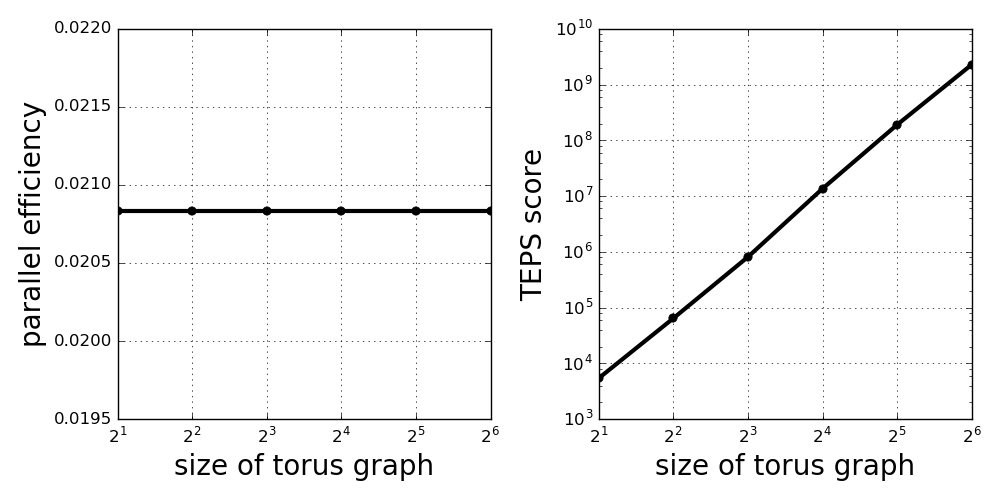
\includegraphics[scale=0.5]{scalegraph.png}
\caption{Parallel efficiency and TEPS score with varying graph size}
\end{figure}

\newpage
\section*{Scaling with number of cores}
\noindent Here, the (torus) graph size was kept fixed at 64x64. The number of BFS traversals were again limited to 100.
\begin{figure}[h!]
\centering
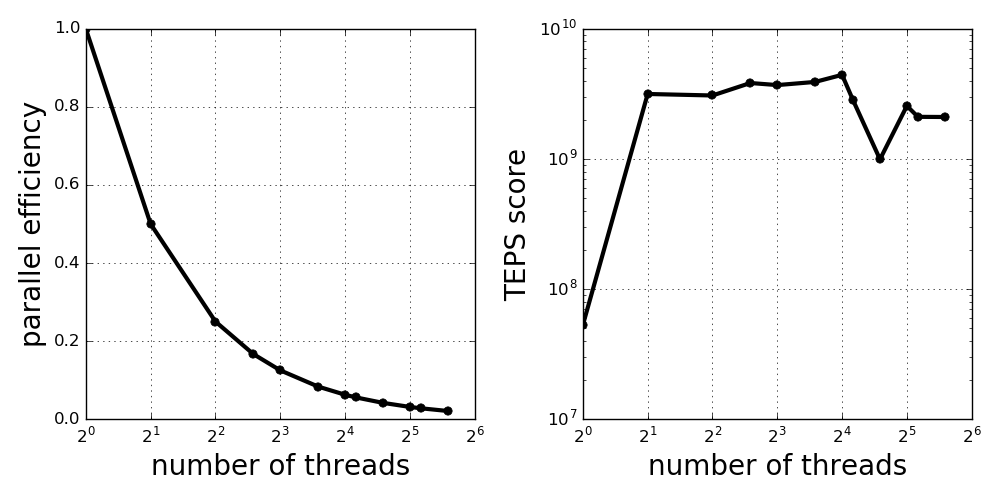
\includegraphics[scale=0.5]{scalecore.png}
\caption{Parallel efficiency and TEPS score with varying thread pool}
\end{figure}

\section*{Discussion}
\noindent For the scaling with number of threads in Fig.2 , I find it surprising that the speedup continues while the TEPS score starts decreasing. The scaling of parallel efficiency with graph size in Fig 1 is bizarre and most probably incorrect, because of all the data racing that I was unable to get rid of. So, while I learnt a lot from this assignment, it is unlikely that either of my scaling results are correct.
\end{document}